\section{Exercice 2}
Le but de cet exercice est de créer un serveur permettant d'afficher ce qu'un client s'y étant connecté lui a envoyé. Ce serveur nous permettra entre autres de voir la syntaxe d'une requête HTTP GET en connectant un navigateur web sur l'adresse et le port du serveur.

\subsection{Client}
Cela n'était pas demandé dans la consigne, mais un client a tout d'abord été créé. Les fonctions écrites ici nous servirons de nouveau par la suite, notamment celle nous permettant d'initialiser une stream socket du côté d'un client.\\

Nous initialisons tout d'abord la stream socket (socket connectée) soit à l'aide de la fonction \emph{init\_stream\_client\_socket()}, soit à l'aide de la fonction \emph{init\_stream\_client\_socket\_alt()}. Ces fonctions définies dans le fichier \emph{socket\_tools.c} servent à initialiser une socket permettant de se connecter à un serveur en utilisant \emph{gethostbyname()} pour la première, et en utilisant \emph{getaddrinfo()} pour la seconde. Celles-ci seront détaillées par la suite. Une fois l'initialisation de la socket effectuée, les caractères écrits sur l'entrée standard sont envoyés un par un au serveur via la socket. La lecture de caractères s'arrête lorsque le caractère EOF (ctrl + d) est tapé.

\begin{lstlisting}
...

sockfd = init_stream_client_socket(argv[1], atoi(argv[2]));

do {
    int sent_size;

    c = getchar();
    sent_size = send(sockfd, &c, 1, 0);
    if (sent_size == -1) {
        perror("client - send");
    }
} while (c != EOF);

...
\end{lstlisting}

\subsubsection{init\_stream\_client\_socket - gethostbyname}
L'initialisation de la socket connectée côté client est similaire à l'initialisation de la datagram socket vue à l'exercice précédent : récupération des informations du serveur à l'aide de \emph{gethostbyname()}, création de la socket (avec \emph{SOCK\_STREAM} et non plus \emph{SOCK\_DGRAM}), et remplissage de la structure \emph{sockaddr\_in}. A cela vient se rajouter l'étape de connexion de la socket à l'aide de l'appel système \emph{connect()} qui prend en paramètres le descripteur de fichier de la socket, l'adresse de la structure précédemment remplie, et sa taille.\\

\begin{lstlisting}
int init_stream_client_socket(const char* hostname, int port) {
    int sockfd, status;
    struct hostent *he;
    struct sockaddr_in dest_addr;

    // Retrieve server information
    he = gethostbyname(hostname);
    if (he == NULL) {
        perror("client - gethostbyname");
        exit(EXIT_FAILURE);
    }

    // Create socket (IPv4, connected, TCP)
    sockfd = socket(AF_INET, SOCK_STREAM, 0);
    if (sockfd == -1) {
        perror("client - socket init");
        exit(EXIT_FAILURE);
    }

    // Fill dest_addr
    dest_addr.sin_family = AF_INET;
    dest_addr.sin_port = htons(port);
    dest_addr.sin_addr = *((struct in_addr*) he->h_addr_list[0]);
    memset(dest_addr.sin_zero, 0, sizeof(dest_addr.sin_zero));

    // Connect the socket
    status = connect(sockfd, (struct sockaddr*) &dest_addr, sizeof(dest_addr));
    if (status == -1) {
        perror("client - connect");
        exit(EXIT_FAILURE);
    }

    return sockfd;
}
\end{lstlisting}

\subsubsection{init\_stream\_client\_socket\_alt - getaddrinfo}
Comme précisé précédemment, l'utilisation de \emph{getaddrinfo()} est aujourd'hui préférée par rapport à \emph{gethostbyname()}. Une alternative à la fonction précédente (initialisation d'une stream socket du côté client) utilisant \emph{getaddrinfo()} a donc été écrite. \emph{getaddrinfo()} possède plusieurs avantage, le premier étant qu'elle fonctionne pour les protocoles IPv4 et IPv6, et le second étant qu'elle permet d'éviter l'étape de remplissage de la structure \emph{sockaddr}, celle-ci est en effet automatiquement remplie. Le premier paramètre est le nom de l'hôte ou son adresse IP, le second est le numéro de port, et le troisième est une structure \emph{addrinfo} qui va permettre de sélectionner les résultats qui nous intéressent. Enfin, le quatrième est une liste de résultats (liste d'\emph{addrinfo}) qui va être remplie par la fonction.\\

\begin{mdframed}[backgroundcolor=lightblue, linecolor=darkblue]
La fonction \emph{getaddrinfo()} ne fait pas partie du standard C99, mais du standard POSIX, il faut donc compiler le programme avec \emph{-D\_POSIX\_SOURCE}.
\end{mdframed}

\begin{lstlisting}
int init_stream_client_socket_alt(const char* hostname, const char *port) {
    int sockfd, status;
    struct addrinfo hints, *res, *tmp;

    memset(&hints, 0, sizeof(hints));
    hints.ai_family = AF_UNSPEC; // IPv4 or IPv6
    hints.ai_socktype = SOCK_STREAM;

    status = getaddrinfo(hostname, port, &hints, &res);
    if (status != 0) {
        fprintf(stderr, "getaddrinfo: %s\n", gai_strerror(status));
        exit(EXIT_FAILURE);
    }

    /* res contains a list of address structures, loop until we successfully
     * connect to the server. */
    for (tmp = res ; tmp != NULL ; tmp = tmp->ai_next) {
        sockfd = socket(tmp->ai_family, tmp->ai_socktype, tmp->ai_protocol);
        if (sockfd == -1) {
            perror("client - socket init");
            continue;
        }

        status = connect(sockfd, tmp->ai_addr, tmp->ai_addrlen);
        if (status == -1) {
            perror("client - connect");
            close(sockfd);
            continue;
        }

        break;
    }

    freeaddrinfo(res);

    if (tmp == NULL) {
        fprintf(stderr, "client - failed to connect to any server\n");
        exit(EXIT_FAILURE);
    }

    return sockfd;
}
\end{lstlisting}

\subsection{Serveur}
Du côté du serveur, la socket est tout d'abord initialisée, une requête de connexion d'un client est attendue et acceptée à l'aide de l'appel système \emph{accept()}, puis on affiche ce qu'a envoyé le client.\\

\begin{lstlisting}
...

sockfd = init_stream_server_socket(atoi(argv[1]));

// Accept one connection request from a client
clientfd = accept(sockfd, NULL, NULL);
if (clientfd == -1) {
    perror("server - accept");
    return EXIT_FAILURE;
}

recv_print_request(clientfd);

...
\end{lstlisting}
\

L'initialisation de la socket est effectuée à l'aide de la fonction \emph{init\_stream\_server\_socket()} définie dans \emph{socket\_tools.c}. Celle-ci prend en paramètre le port sur lequel la socket va être liée. La socket est d'abord créée à l'aide de l'appel système \emph{socket()}. Une structure \emph{sockaddr\_in} est ensuite remplie, celle-ci va nous servir à lier la socket à l'aide de \emph{bind()}. Nous spécifions que nous souhaitons que la socket soit liée à toutes les interfaces (\emph{INADDR\_ANY}), et au port passé en paramètre. Enfin, cette socket jouant un role de serveur, celle-ci doit être marquée comme une socket passive (ou encore socket d'écoute) afin d'accepter des requêtes de connexion par la suite.\\

\begin{lstlisting}
int init_stream_server_socket(int port) {
    int sockfd, status;
    struct sockaddr_in serv_addr;

    // Create socket (IPv4, connected, TCP)
    sockfd = socket(AF_INET, SOCK_STREAM, 0);
    if (sockfd == -1) {
        perror("server - socket init");
        exit(EXIT_FAILURE);
    }

    // Fill serv_addr
    serv_addr.sin_family = AF_INET;
    serv_addr.sin_port = htons(port);
    serv_addr.sin_addr.s_addr = INADDR_ANY;
    memset(serv_addr.sin_zero, 0, sizeof(serv_addr.sin_zero));

    // Bind socket to all local interfaces on the port specified in argument
    status = bind(sockfd, (struct sockaddr *) &serv_addr, sizeof(serv_addr));
    if (status == -1) {
        perror("server - bind");
        exit(EXIT_FAILURE);
    }

    // Passive (listening) socket
    status = listen(sockfd, 1);
    if (status == -1) {
        perror("server - listen");
        exit(EXIT_FAILURE);
    }

    return sockfd;
}
\end{lstlisting}
\

Enfin, on reçoit les messages envoyés par le client à l'aide de \emph{read()} et on les affiche jusqu'à ce qu'il n'y ait plus rien à lire ou que {\textbackslash r \textbackslash n \textbackslash r \textbackslash n} (indication de fin d'une requête HTTP) soit lu. Cette dernière étape est réalisée par la fonction \emph{recv\_print\_request} définie dans le fichier \emph{http\_tools.c}.

\subsection{Requête HTTP}
On souhaite récupérer la syntaxe d'une requête HTTP à l'aide d'un navigateur web, et du serveur écrit pour cet exercice. Pour cela, le serveur est lancé sur un port (e.g 10000) et une requête est lancé depuis le navigateur à destination de \emph{localhost:10000}. Ci-dessous un exemple de requête reçue.

\begin{figure}[h!]
	\centering
	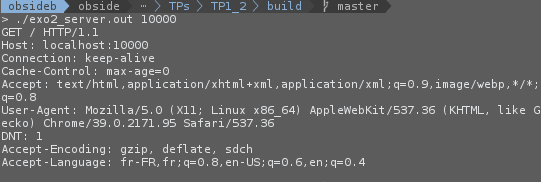
\includegraphics[width=0.8\textwidth]{screenshots/ex2.png}
	\caption{exo2\_server.out - récupération d'une requête HTTP}
\end{figure}

La deux premières lignes de cette requête sont les plus importantes, la première indique que l'on souhaite obtenir la ressource / et que l'on utilise le protocole HTTP/1.1. La seconde ligne indique que la requête est à destination de l'hôte localhost sur le port 10000. Les autres lignes sont optionnelles, et indiquent par exemple de quel navigateur provient la requête, ou encore quels types de fichiers sont acceptés. Les sauts de lignes dans une requête HTTP sont composés d'un retour chariot (\textbackslash r) et d'une nouvelle ligne (\textbackslash n), la dernière ligne étant signalée par deux sauts de ligne (\textbackslash r \textbackslash n \textbackslash r \textbackslash n).
